\chapter{Les ions et les solutions ioniques}\label{ch:g9:ions}

Deux boissons limpides sont posées sur un banc de gymnase~: une bouteille
de boisson pour sportifs, vendue pour ses «~électrolytes~», et un verre
d'eau sucrée. Au laboratoire, on plonge tour à tour dans chacune deux
plaques de métal reliées à une pile et à une petite lampe. Dans la
boisson pour sportifs, la lampe s'allume~; dans l'eau sucrée, elle reste
éteinte. Quelque chose, dans le premier liquide, transporte des charges
électriques, et le sucre, non. Ce quelque chose, ce sont des \omterm{def:g9:ions:ion}{ions}.

\begin{recall}
Un \omterm{def:g7:atoms-and-molecules:atom}{atome} possède un \omterm{def:g9:inside-the-atom:nucleus}{noyau} de $Z$ \omterm{def:g9:inside-the-atom:proton}{protons}, chacun de charge $+e$, et $Z$
\omterm{def:g9:inside-the-atom:nucleus}{électrons} autour de lui, chacun de charge $-e$~: l'\omterm{def:g7:atoms-and-molecules:atom}{atome} est neutre
(\cref{ch:g9:inside-the-atom}). Un \omterm{def:g6:solutions-and-solubility:solute}{soluté} dissous dans l'eau donne une
\omterm{def:g6:solutions-and-solubility:solute}{solution aqueuse} (\cref{ch:g6:solutions-and-solubility}). Un \omterm{def:g7:identifying-substances:characteristic-test}{test
caractéristique} détecte une espèce par un résultat visible
(\cref{ch:g7:identifying-substances}).
\end{recall}

\begin{omfigure}
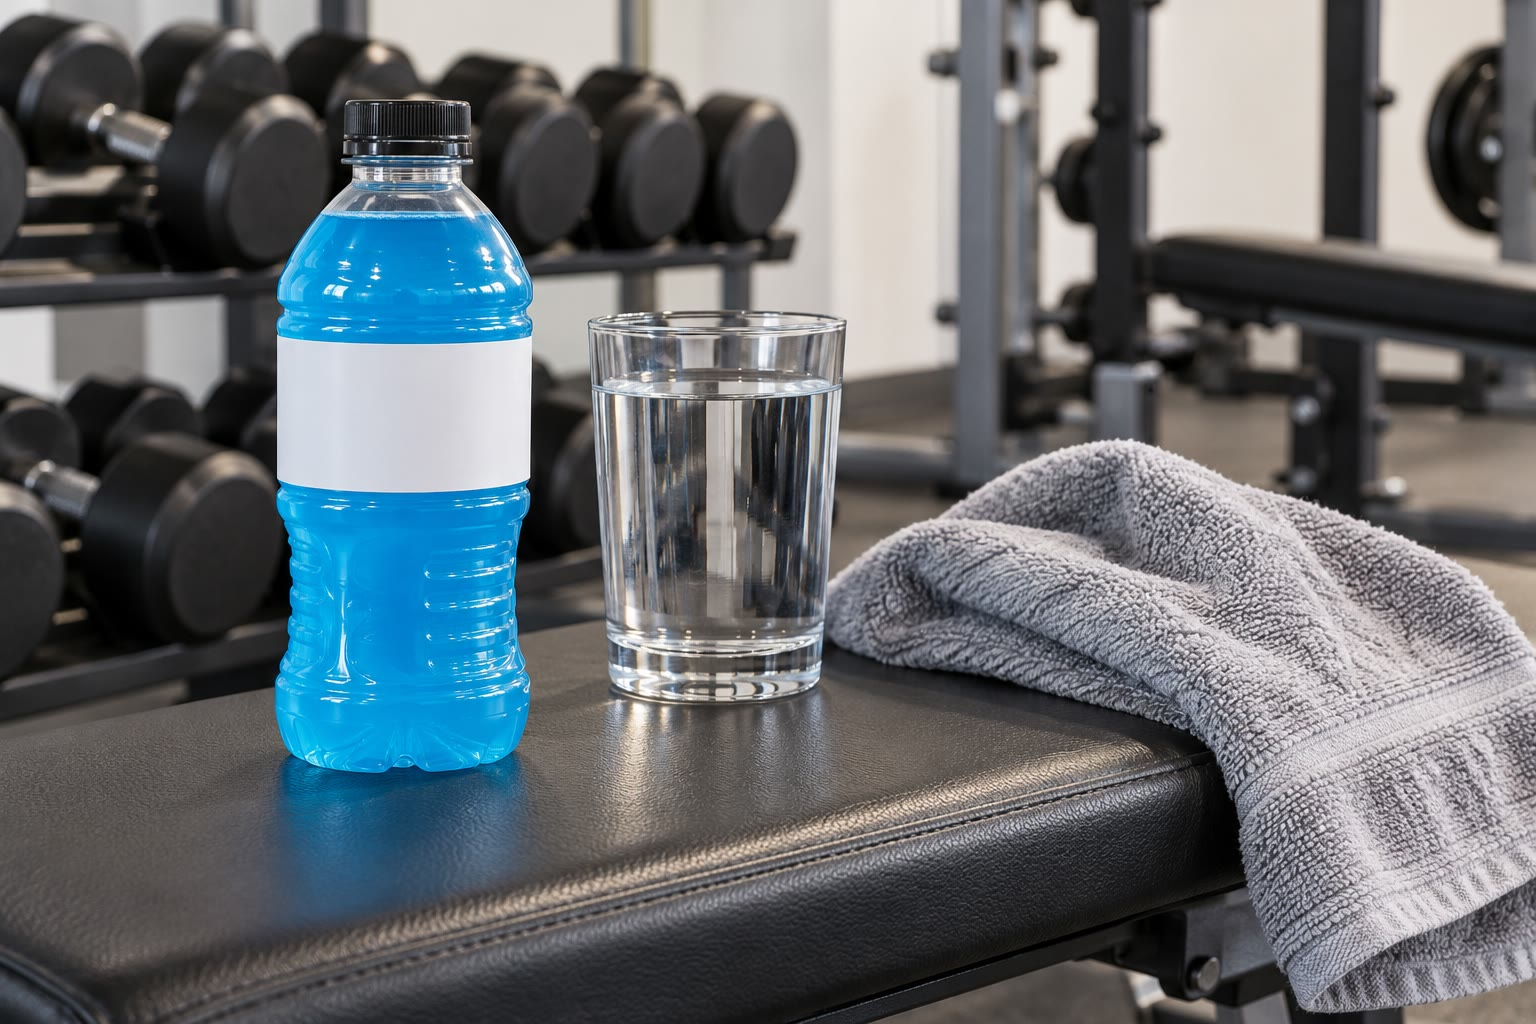
\includegraphics[width=0.5\linewidth]{images/book1/ai/g9-sports-drink.jpg}

{\small Une boisson pour sportifs et un verre d'eau~: la boisson contient
des \omterm{def:g9:ions:ion}{ions} dissous.}
\end{omfigure}

\section{Des atomes qui gagnent ou perdent des électrons}

\begin{definition}[Ion, cation, anion]\label{def:g9:ions:ion}
Un \emph{ion}\index{ion} est un \omterm{def:g7:atoms-and-molecules:atom}{atome}, ou un groupe d'\omterm{def:g7:atoms-and-molecules:atom}{atomes}, qui a perdu
ou gagné un ou plusieurs \omterm{def:g9:inside-the-atom:nucleus}{électrons}, et qui porte donc une charge
électrique. Un ion de charge positive, qui a perdu des \omterm{def:g9:inside-the-atom:nucleus}{électrons}, est un
\emph{cation}\index{cation}~; un ion de charge négative, qui a gagné des
\omterm{def:g9:inside-the-atom:nucleus}{électrons}, est un \emph{anion}\index{anion}. La charge s'écrit en haut à
droite de la formule~: \ce{Na+}, \ce{Cu^{2+}}, \ce{Cl-}.
\end{definition}

\begin{example}[Le sodium et le chlore]\label{ex:g9:ions:na-cl}
Un \omterm{def:g7:atoms-and-molecules:atom}{atome} de sodium, 11 \omterm{def:g9:inside-the-atom:proton}{protons} et 11 \omterm{def:g9:inside-the-atom:nucleus}{électrons}, perd un \omterm{def:g9:inside-the-atom:nucleus}{électron}~: il
devient l'\omterm{def:g9:ions:ion}{ion} sodium \ce{Na+}, 11 \omterm{def:g9:inside-the-atom:proton}{protons} et 10 \omterm{def:g9:inside-the-atom:nucleus}{électrons}, de charge
$+1$~:
\[
  \ce{Na -> Na+ + e-}.
\]
Un \omterm{def:g7:atoms-and-molecules:atom}{atome} de chlore, 17 \omterm{def:g9:inside-the-atom:proton}{protons} et 17 \omterm{def:g9:inside-the-atom:nucleus}{électrons}, gagne un \omterm{def:g9:inside-the-atom:nucleus}{électron}~: il
devient l'\omterm{def:g9:ions:ion}{ion} chlorure \ce{Cl-}, 17 \omterm{def:g9:inside-the-atom:proton}{protons} et 18 \omterm{def:g9:inside-the-atom:nucleus}{électrons}~:
\[
  \ce{Cl + e- -> Cl-}.
\]
\end{example}

\begin{omfigure}
\begin{tikzpicture}[font=\small]
  \foreach \x/\name/\p/\e/\ch/\col in {0/{atome de sodium}/11/11/0/omDef,
      3.7/{ion sodium \ce{Na+}}/11/10/+1/omProp,
      8.0/{atome de chlore}/17/17/0/omDef, 11.7/{ion chlorure \ce{Cl-}}/17/18/$-1$/omProp} {
    \node[draw=\col, fill=\col!6, rounded corners=2pt, align=center, text width=2.4cm]
      at (\x,0) {\textbf{\name}\\ \p\ protons\\ \e\ électrons\\ charge \ch};
  }
  \draw[->, thick, omProp] (1.45,0) -- (2.25,0) node[midway, above, text=black,
    font=\footnotesize, align=center] {perd\\ 1 \ce{e-}};
  \draw[->, thick, omProp] (9.45,0) -- (10.25,0) node[midway, above, text=black,
    font=\footnotesize, align=center] {gagne\\ 1 \ce{e-}};
\end{tikzpicture}

{\small Un \omterm{def:g7:atoms-and-molecules:atom}{atome} de sodium devient un \omterm{def:g9:ions:ion}{ion} sodium en perdant un
\omterm{def:g9:inside-the-atom:nucleus}{électron}~; un \omterm{def:g7:atoms-and-molecules:atom}{atome} de chlore devient un \omterm{def:g9:ions:ion}{ion} chlorure en en gagnant un.
Les \omterm{def:g9:inside-the-atom:proton}{protons} ne changent pas.}
\end{omfigure}

\begin{proposition}[Quelques ions courants]\label{prop:g9:ions:common}
Les \omterm{def:g9:ions:ion}{ions} monoatomiques sont formés à partir d'un seul \omterm{def:g7:atoms-and-molecules:atom}{atome}~; les \omterm{def:g9:ions:ion}{ions}
polyatomiques, à partir d'un groupe d'\omterm{def:g7:atoms-and-molecules:atom}{atomes} qui reste uni~:
\begin{center}
\small
\begin{tabular}{llll}
\hline
\omterm{def:g9:ions:ion}{cations} & & \omterm{def:g9:ions:ion}{anions} & \\
\hline
sodium & \ce{Na+} & chlorure & \ce{Cl-} \\
potassium & \ce{K+} & hydroxyde & \ce{OH-} \\
calcium & \ce{Ca^{2+}} & nitrate & \ce{NO3-} \\
magnésium & \ce{Mg^{2+}} & carbonate & \ce{CO3^{2-}} \\
cuivre(II) & \ce{Cu^{2+}} & sulfate & \ce{SO4^{2-}} \\
fer(II), fer(III) & \ce{Fe^{2+}}, \ce{Fe^{3+}} & & \\
zinc & \ce{Zn^{2+}} & & \\
aluminium & \ce{Al^{3+}} & & \\
ammonium & \ce{NH4+} & & \\
\hline
\end{tabular}
\end{center}
\end{proposition}

\section{Les composés ioniques et leurs formules}

\begin{definition}[Composé ionique]\label{def:g9:ions:ionic-compound}
Un \emph{composé ionique}\index{compose ionique@composé ionique} est formé de \omterm{def:g9:ions:ion}{cations} et
d'\omterm{def:g9:ions:ion}{anions} en nombres tels que l'ensemble ne porte aucune charge. Sa
formule donne la proportion des \omterm{def:g9:ions:ion}{ions}, sans leurs charges~: \ce{NaCl}
pour le chlorure de sodium, un \ce{Na+} pour chaque \ce{Cl-}~;
\ce{CaCl2} pour le chlorure de calcium, deux \ce{Cl-} pour chaque
\ce{Ca^{2+}}.
\end{definition}

\begin{method}[Écrire la formule d'un composé ionique]\label{met:g9:ions:formula}
\begin{enumerate}
  \item Écrire les deux \omterm{def:g9:ions:ion}{ions} avec leurs charges, le \omterm{def:g9:ions:ion}{cation} d'abord.
  \item Trouver les plus petits nombres de chacun qui rendent la charge
        totale nulle.
  \item Écrire ces nombres en \omterm{def:g7:atoms-and-molecules:formula}{indice}~; un \omterm{def:g9:ions:ion}{ion} polyatomique qui a besoin
        d'un \omterm{def:g7:atoms-and-molecules:formula}{indice} se met entre parenthèses.
\end{enumerate}
Oxyde d'aluminium~: \ce{Al^{3+}} et \ce{O^{2-}}~; $2 \times (+3) + 3 \times
(-2) = 0$, donc \ce{Al2O3}. Hydroxyde de fer(III)~: \ce{Fe^{3+}} et trois
\ce{OH-}~: \ce{Fe(OH)3}.
\end{method}

\begin{proposition}[Un solide ionique est un empilement d'ions]\label{prop:g9:ions:solid}
Dans un cristal de sel, les \omterm{def:g9:ions:ion}{ions} sodium et les \omterm{def:g9:ions:ion}{ions} chlorure alternent
en un empilement régulier à trois dimensions, chaque \omterm{def:g9:ions:ion}{ion} étant entouré
d'\omterm{def:g9:ions:ion}{ions} de charge opposée qui le maintiennent en place. Un grain de sel
de table en contient des milliards de milliards~; sa forme cubique
reflète l'empilement cubique.
\end{proposition}

\begin{omfigure}
\begin{minipage}[b]{0.5\linewidth}\centering
\begin{tikzpicture}[font=\small]
  \foreach \i in {0,...,5} \foreach \j in {0,...,4} {
    \pgfmathtruncatemacro\pp{mod(\i+\j,2)}
    \ifnum\pp=0 \node[aNa, minimum size=5mm] at (0.62*\i,0.62*\j) {};
    \else \node[aCl, minimum size=7.4mm] at (0.62*\i,0.62*\j) {};\fi
  }
\end{tikzpicture}

{\small Une couche d'un cristal de sel~: les \omterm{def:g9:ions:ion}{ions} sodium (violets, plus
petits) et les \omterm{def:g9:ions:ion}{ions} chlorure (verts) alternent.}
\end{minipage}\hfill
\begin{minipage}[b]{0.3\linewidth}\centering
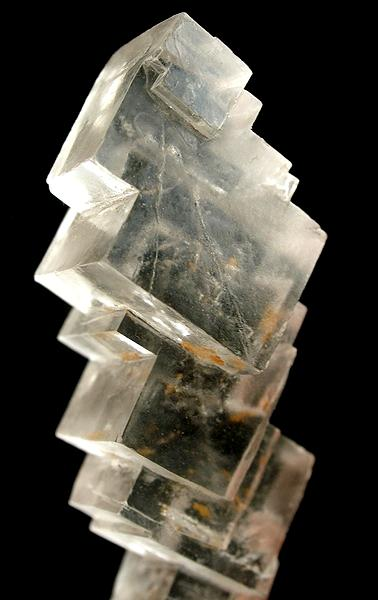
\includegraphics[height=4.6cm]{images/book1/halite.jpg}

{\small La halite, le sel gemme naturel. Photo~: Robert M.~Lavinsky,
CC BY-SA 3.0.}
\end{minipage}
\end{omfigure}

\section{Les solutions ioniques conduisent le courant}

\begin{notation}[Le symbole d'état (aq)]\label{not:g9:ions:aq}
Un \omterm{def:g9:ions:ion}{ion} ou une \omterm{def:g7:atoms-and-molecules:molecule}{molécule} dissous dans l'eau est noté (aq), pour
«~aqueux~»~: \ce{Na+(aq)}, \ce{Cl-(aq)}.
\end{notation}

\begin{proposition}[Les solutions ioniques conduisent l'électricité]\label{prop:g9:ions:conduct}
Quand un \omterm{def:g9:ions:ionic-compound}{composé ionique} \omterm{def:g2:mixing-and-dissolving:dissolve}{se dissout} dans l'eau, ses \omterm{def:g9:ions:ion}{ions} se séparent et
se déplacent librement dans la solution~: l'eau salée contient des
\ce{Na+(aq)} et des \ce{Cl-(aq)}. Des \omterm{def:g9:ions:ion}{ions} en mouvement transportent des
charges électriques~: une solution ionique conduit donc l'électricité.
Une solution de sucre, dont les \omterm{def:g7:atoms-and-molecules:molecule}{molécules} ne portent pas de charge, ne
la conduit pas~; l'eau très pure non plus.
\end{proposition}

\begin{inthelab}[Quels liquides conduisent~?]
L'enseignant monte en circuit deux plaques de métal, une pile de faible
tension et une petite lampe~; on plonge les plaques tour à tour dans de
l'eau distillée, de l'eau sucrée, de l'eau salée et une solution de
sulfate de cuivre, en les rinçant entre chaque essai. La lampe ne
s'allume qu'avec les deux solutions ioniques.
\end{inthelab}

\begin{omfigure}
\begin{tikzpicture}[font=\small, scale=1.1]
  \foreach \xs/\lit/\lab in {0/1/{eau salée~: la lampe s'allume}, 5.2/0/{eau sucrée~: elle reste éteinte}} {
    \begin{scope}[xshift=\xs cm]
      \pic[transform shape] at (2,0) {beaker={0.7}{omWater!80}};
      \fill[black!45] (1.6,0.25) rectangle (1.7,2.6);
      \fill[black!45] (2.3,0.25) rectangle (2.4,2.6);
      \ifnum\lit=1 \fill[yellow!70, opacity=0.8] (3.4,3.0) circle (0.42);\fi
      \draw (1.65,2.6) -- (1.65,3.6) to[battery1] (3.4,3.6) -- (3.4,3.4)
        to[lamp] (3.4,2.6) -- (2.35,2.6);
      \node[anchor=north, align=center] at (2,-0.15) {\lab};
    \end{scope}
  }
\end{tikzpicture}

{\small Le test de conduction~: avec l'eau salée, les \omterm{def:g9:ions:ion}{ions} transportent
le courant et la lampe s'allume~; l'eau sucrée ne contient pas d'\omterm{def:g9:ions:ion}{ions} et
la lampe reste éteinte.}
\end{omfigure}

\section{Les tests de reconnaissance des ions par précipitation}

\begin{definition}[Précipité]\label{def:g9:ions:precipitate}
Quand on \omterm{def:g6:pure-substances-and-mixtures:mixture}{mélange} deux solutions, un \omterm{def:g9:ions:ion}{cation} de l'une et un \omterm{def:g9:ions:ion}{anion} de
l'autre peuvent former un \omterm{def:g9:ions:ionic-compound}{composé ionique} qui ne \omterm{def:g2:mixing-and-dissolving:dissolve}{se dissout} pas. Il
apparaît sous forme d'un solide fin qui trouble le liquide et se dépose~:
c'est un \emph{précipité}\index{precipite@précipité}. La réaction est une
\emph{précipitation}\index{precipitation@précipitation}.
\end{definition}

\begin{proposition}[Les tests des ions courants]\label{prop:g9:ions:tests}
Quelques gouttes d'une solution de \omterm{def:g7:chemical-reactions:reactant}{réactif} identifient un \omterm{def:g9:ions:ion}{ion} par la
couleur du \omterm{def:g9:ions:precipitate}{précipité} qu'il forme~:
\begin{center}
\small
\begin{tabular}{llll}
\hline
\omterm{def:g9:ions:ion}{ion} recherché & \omterm{def:g7:chemical-reactions:reactant}{réactif} & \omterm{def:g9:ions:precipitate}{précipité} & couleur \\
\hline
cuivre(II) \ce{Cu^{2+}} & hydroxyde de sodium & \ce{Cu(OH)2} & bleu \\
fer(II) \ce{Fe^{2+}} & hydroxyde de sodium & \ce{Fe(OH)2} & vert \\
fer(III) \ce{Fe^{3+}} & hydroxyde de sodium & \ce{Fe(OH)3} & rouille \\
zinc \ce{Zn^{2+}} & hydroxyde de sodium & \ce{Zn(OH)2} & blanc \\
aluminium \ce{Al^{3+}} & hydroxyde de sodium & \ce{Al(OH)3} & blanc \\
chlorure \ce{Cl-} & nitrate d'argent & \ce{AgCl} & blanc, noircit à la lumière \\
\hline
\end{tabular}
\end{center}
\end{proposition}

\begin{example}[Écrire une précipitation]\label{ex:g9:ions:equation}
On n'écrit que les \omterm{def:g9:ions:ion}{ions} qui forment le solide~; les autres restent
dissous et ne participent pas~:
\[
  \ce{Cu^{2+}(aq) + 2OH-(aq) -> Cu(OH)2(s)}, \qquad
  \ce{Ag+(aq) + Cl-(aq) -> AgCl(s)}.
\]
\end{example}

\begin{omfigure}
\begin{tikzpicture}[font=\small, scale=0.95]
  \foreach \k/\pc/\lab in {0/blue!60/{\ce{Cu^{2+}}~: bleu}, 1/green!45!black!70/{\ce{Fe^{2+}}~: vert},
      2/orange!70!brown/{\ce{Fe^{3+}}~: rouille}, 3/white!85!black/{\ce{Zn^{2+}}~: blanc},
      4/white!85!black/{\ce{Al^{3+}}~: blanc}, 5/white!80!black/{\ce{Cl-}~: blanc}} {
    \pic[transform shape] at (\k*2.3,0) {testtube={0.5}{omWater!60}};
    \pic[transform shape] at (\k*2.3,0) {testtube={0.14}{\pc}};
    \node[anchor=north, align=center, font=\footnotesize, text width=2cm] at (\k*2.3,-0.15) {\lab};
  }
\end{tikzpicture}

{\small Les \omterm{def:g9:ions:precipitate}{précipités} formés avec l'hydroxyde de sodium (les cinq
premiers tubes) et avec le nitrate d'argent (le dernier tube).}
\end{omfigure}

\begin{safety}{\ghs[0.82cm]{GHS05}\ghs[0.82cm]{GHS07}}
% ledger: ghs:NaOH, ghs:AgNO3
L'hydroxyde de sodium provoque de graves brûlures de la peau et des
lésions oculaires, et peut être corrosif pour les métaux (GHS05)~; dilué,
il est irritant pour la peau et les yeux (GHS07). Le nitrate d'argent,
le \omterm{def:g7:chemical-reactions:reactant}{réactif} des \omterm{def:g9:ions:ion}{ions} chlorure, est comburant, corrosif et très toxique
pour les organismes aquatiques. Lunettes, gants~; les \omterm{def:g7:chemical-reactions:reactant}{réactifs} sont
distribués goutte à goutte par l'enseignant.
\end{safety}

\begin{method}[Tester un ion]\label{met:g9:ions:test}
\begin{enumerate}
  \item Verser un peu de la solution à tester dans un tube à essai.
  \item Ajouter le \omterm{def:g7:chemical-reactions:reactant}{réactif} goutte à goutte.
  \item Noter la couleur du \omterm{def:g9:ions:precipitate}{précipité} éventuel et la comparer au
        tableau.
  \item Conclure, en se rappelant qu'un test identifie un \omterm{def:g9:ions:ion}{ion}, et non un
        composé~: une solution de chlorure de fer(III) donne à la fois le
        test de \ce{Fe^{3+}} et celui de \ce{Cl-}.
\end{enumerate}
\end{method}

\section{Exercices}

\begin{exercise}[$\star$]\label{exo:g9:ions:1}
Qu'est-ce qu'un \omterm{def:g9:ions:ion}{ion}~? Quelle est la différence entre un \omterm{def:g9:ions:ion}{cation} et un
\omterm{def:g9:ions:ion}{anion}~?
\end{exercise}

\begin{exercise}[$\star$]\label{exo:g9:ions:2}
Un \omterm{def:g7:atoms-and-molecules:atom}{atome} de magnésium (12 \omterm{def:g9:inside-the-atom:proton}{protons}) perd deux \omterm{def:g9:inside-the-atom:nucleus}{électrons}. Écris la
formule de l'\omterm{def:g9:ions:ion}{ion} formé, et donne ses nombres de \omterm{def:g9:inside-the-atom:proton}{protons} et d'\omterm{def:g9:inside-the-atom:nucleus}{électrons}.
\end{exercise}

\begin{exercise}[$\star$]\label{exo:g9:ions:3}
Écris les formules du chlorure de potassium, du chlorure de magnésium et
de l'oxyde de calcium (\omterm{def:g9:ions:ion}{ion} oxyde~: \ce{O^{2-}}).
\end{exercise}

\begin{exercise}[$\star$]\label{exo:g9:ions:4}
Pourquoi l'eau salée conduit-elle l'électricité, alors que l'eau sucrée
ne la conduit pas~?
\end{exercise}

\begin{exercise}[$\star\star$]\label{exo:g9:ions:5}
Écris les formules du sulfate de cuivre(II), du chlorure d'aluminium et
du carbonate de sodium.
\end{exercise}

\begin{exercise}[$\star\star$]\label{exo:g9:ions:6}
L'hydroxyde de sodium ajouté à une solution donne un \omterm{def:g9:ions:precipitate}{précipité} rouille.
Quel \omterm{def:g9:ions:ion}{ion} la solution contient-elle~? Écris l'équation de la
\omterm{def:g9:ions:precipitate}{précipitation}.
\end{exercise}

\begin{exercise}[$\star\star$]\label{exo:g9:ions:7}
Combien d'\omterm{def:g9:inside-the-atom:nucleus}{électrons} l'\omterm{def:g9:ions:ion}{ion} sulfate \ce{SO4^{2-}} porte-t-il en plus de
ses \omterm{def:g9:inside-the-atom:proton}{protons}~? Et l'\omterm{def:g9:ions:ion}{ion} nitrate \ce{NO3-}~?
\end{exercise}

\begin{exercise}[$\star\star$]\label{exo:g9:ions:8}
Une solution donne un \omterm{def:g9:ions:precipitate}{précipité} blanc avec le nitrate d'argent et un
\omterm{def:g9:ions:precipitate}{précipité} bleu avec l'hydroxyde de sodium. Nomme le \omterm{def:g9:ions:ionic-compound}{composé ionique}
dissous et écris sa formule.
\end{exercise}

\begin{exercise}[$\star\star$]\label{exo:g9:ions:9}
Regarde la figure de la couche du cristal de sel. Combien de voisins de
charge opposée un \omterm{def:g9:ions:ion}{ion} situé au milieu de la couche a-t-il dans cette
couche~?
\end{exercise}

\begin{exercise}[$\star\star$]\label{exo:g9:ions:10}
Écris l'équation de la \omterm{def:g9:ions:precipitate}{précipitation} de l'hydroxyde de fer(II) à partir
des \omterm{def:g9:ions:ion}{ions} \ce{Fe^{2+}} et \ce{OH-}.
\end{exercise}

\begin{exercise}[$\star\star\star$]\label{exo:g9:ions:11}
Une poudre blanche peut être du chlorure de zinc ou du chlorure de
sodium. Dissoute dans l'eau, elle donne un \omterm{def:g9:ions:precipitate}{précipité} blanc avec
l'hydroxyde de sodium. Laquelle est-ce~? Écris l'équation.
\end{exercise}

\begin{exercise}[$\star\star\star$]\label{exo:g9:ions:12}
Dans un cristal de chlorure de calcium, combien y a-t-il d'\omterm{def:g9:ions:ion}{ions} chlorure
pour 1000 \omterm{def:g9:ions:ion}{ions} calcium~? Vérifie que le cristal est neutre.
\end{exercise}

\section{Problème~: le puits rouillé}

\begin{problem}[{Problème du week-end --- des taches orange dans l'évier
d'une ferme, deux tests, et le nombre d'ions fer dans un litre d'eau de
puits}]
\label{pb:g9:ions:1}
L'eau du puits d'une ferme laisse des taches orange dans l'évier. Un
laboratoire en reçoit un échantillon. Fraîchement tirée, l'eau est
limpide~; avec l'hydroxyde de sodium, elle donne un \omterm{def:g9:ions:precipitate}{précipité} vert, qui
devient rouille en moins d'une heure à la surface, au contact de l'\omterm{def:g4:air-a-mixture-of-gases:air}{air}.
Le laboratoire mesure \qty{0.30}{mg} de fer, sous forme d'\omterm{def:g9:ions:ion}{ions} fer, par
litre. On prendra pour masse d'un \omterm{def:g9:inside-the-atom:proton}{nucléon} \qty{1.67e-27}{kg}, et
56 \omterm{def:g9:inside-the-atom:proton}{nucléons} pour un \omterm{def:g7:atoms-and-molecules:atom}{atome} de fer.

\medskip
\noindent\textbf{Partie I --- Les tests.}
\begin{enumerate}
  \item Quel \omterm{def:g9:ions:ion}{ion} le \omterm{def:g9:ions:precipitate}{précipité} vert révèle-t-il~? Donne la formule du
        \omterm{def:g9:ions:precipitate}{précipité}.
  \item Quel \omterm{def:g9:ions:ion}{ion} le \omterm{def:g9:ions:precipitate}{précipité} rouille révèle-t-il~? Donne sa formule.
  \item Un \omterm{def:g9:ions:ion}{ion} fer(II) et un \omterm{def:g9:ions:ion}{ion} fer(III) diffèrent d'un \omterm{def:g9:inside-the-atom:nucleus}{électron}.
        Lequel a le plus d'\omterm{def:g9:inside-the-atom:nucleus}{électrons}~? Combien d'\omterm{def:g9:inside-the-atom:nucleus}{électrons} chacun
        possède-t-il (fer~: $Z = 26$)~?
  \item Écris l'équation de la \omterm{def:g9:ions:precipitate}{précipitation} de l'hydroxyde de fer(III).
\end{enumerate}

\medskip
\noindent\textbf{Partie II --- Les taches.}
\begin{enumerate}[resume]
  \item Dans l'évier, l'eau limpide se trouble lentement et devient
        orange. Quel \omterm{def:g9:ions:ion}{ion} l'eau contient-elle à la sortie du puits, et
        lequel finit-elle par contenir~?
  \item Écris la formule du \omterm{def:g9:ions:ionic-compound}{composé ionique} formé par les \omterm{def:g9:ions:ion}{ions} fer(III)
        et les \omterm{def:g9:ions:ion}{ions} hydroxyde, et vérifie qu'il est neutre.
  \item Peut-on retirer le fer de l'eau en la filtrant à la sortie du
        puits~? Après qu'elle est devenue orange~? Explique.
  \item Une eau qui contient des \omterm{def:g9:ions:ion}{ions} fer est-elle un \omterm{def:g6:pure-substances-and-mixtures:pure-substance}{corps pur}~? Un
        \omterm{def:g6:pure-substances-and-mixtures:homogeneous}{mélange homogène}~?
\end{enumerate}

\medskip
\noindent\textbf{Partie III --- Compter les \omterm{def:g9:ions:ion}{ions}.}
\begin{enumerate}[resume]
  \item Calcule la masse d'un \omterm{def:g7:atoms-and-molecules:atom}{atome} de fer, en kilogrammes.
  \item Convertis \qty{0.30}{mg} en kilogrammes.
  \item Pourquoi peut-on prendre la masse d'un \omterm{def:g9:ions:ion}{ion} fer égale à celle d'un
        \omterm{def:g7:atoms-and-molecules:atom}{atome} de fer~?
  \item Calcule le nombre d'\omterm{def:g9:ions:ion}{ions} fer dans un litre de l'eau du puits.
\end{enumerate}
\end{problem}
